\documentclass[aspectratio=169]{beamer}

\mode<presentation>
{
  \usetheme{default}
  \usecolortheme{default}
  \usefonttheme{default}
  \setbeamertemplate{navigation symbols}{}
  \setbeamertemplate{caption}[numbered]
  \setbeamertemplate{footline}[frame number]  % or "page number"
  \setbeamercolor{frametitle}{fg=white}
  \setbeamercolor{footline}{fg=black}
} 

\usepackage[english]{babel}
\usepackage[utf8x]{inputenc}
\usepackage{tikz}
\usepackage{courier}
\usepackage{array}
\usepackage{bold-extra}
\usepackage{minted}
\usepackage[thicklines]{cancel}
\usepackage{fancyvrb}

\xdefinecolor{dianablue}{rgb}{0.18,0.24,0.31}
\xdefinecolor{darkblue}{rgb}{0.1,0.1,0.7}
\xdefinecolor{darkgreen}{rgb}{0,0.5,0}
\xdefinecolor{darkgrey}{rgb}{0.35,0.35,0.35}
\xdefinecolor{darkorange}{rgb}{0.8,0.5,0}
\xdefinecolor{darkred}{rgb}{0.7,0,0}
\definecolor{darkgreen}{rgb}{0,0.6,0}
\definecolor{mauve}{rgb}{0.58,0,0.82}

\definecolor{mycolor}{HTML}{FF6600}
\definecolor{cppcolor}{HTML}{00AAD4}
\definecolor{rootcolor}{HTML}{2A2AFF}
\definecolor{rootnpcolor}{HTML}{008000}
\definecolor{pythoncolor}{HTML}{FF00CC}

\title[2018-07-10-chep-columnar]{Columnar data processing for HEP analysis}

\author[shortname]{Peter Elmer\inst{a} \and \textcolor{darkblue}{Jim Pivarski}\inst{a} \and David Lange\inst{a} \and Jaydeep Nandi\inst{b}}
\institute[shortinst]{\inst{a} Princeton University \and \inst{b} National Institute of Technology, Silchar, India}
\date{July 10, 2018}

\begin{document}

\logo{\pgfputat{\pgfxy(0.11, 7.4)}{\pgfbox[right,base]{\tikz{\filldraw[fill=dianablue, draw=none] (0 cm, 0 cm) rectangle (50 cm, 1 cm);}\mbox{\hspace{-8 cm}
\includegraphics[height=1 cm]{princeton-logo-long.png}
\includegraphics[height=1 cm]{diana-hep-logo-long.png}}}}}

\begin{frame}
  \titlepage
\end{frame}

\logo{\pgfputat{\pgfxy(0.11, 7.4)}{\pgfbox[right,base]{\tikz{\filldraw[fill=dianablue, draw=none] (0 cm, 0 cm) rectangle (50 cm, 1 cm);}\mbox{\hspace{-8 cm}
\includegraphics[height=1 cm]{princeton-logo.png}
\includegraphics[height=1 cm]{diana-hep-logo.png}}}}}

% Uncomment these lines for an automatically generated outline.
%\begin{frame}{Outline}
%  \tableofcontents
%\end{frame}

% START START START START START START START START START START START START START

\begin{frame}{Motivation}
\vspace{0.5 cm}
\large
In the late stages of data analysis, only order-of-magnitude speedups translate into increased human productivity, and only if they're easy to set up.

\vspace{0.5 cm}
\uncover<2->{Producing a plot in a second instead of an hour is life-changing, but not if it takes two hours to write the script.}
\end{frame}

\begin{frame}{Motivation}
\begin{columns}
\column{0.41\linewidth}
However, most HEP analysis doesn't optimize for the most critical performance bottleneck: data layout in memory.

\vspace{0.5 cm}
Modern processors are much faster than memory, so arranging data for dense, sequential scanning is critical. \textcolor{gray}{(a.k.a.\ ``struct of arrays'')}

\vspace{0.5 cm}
However, it can be hard to set up and analyze data in this form.
\column{0.55\linewidth}
\vspace{0.3 cm}
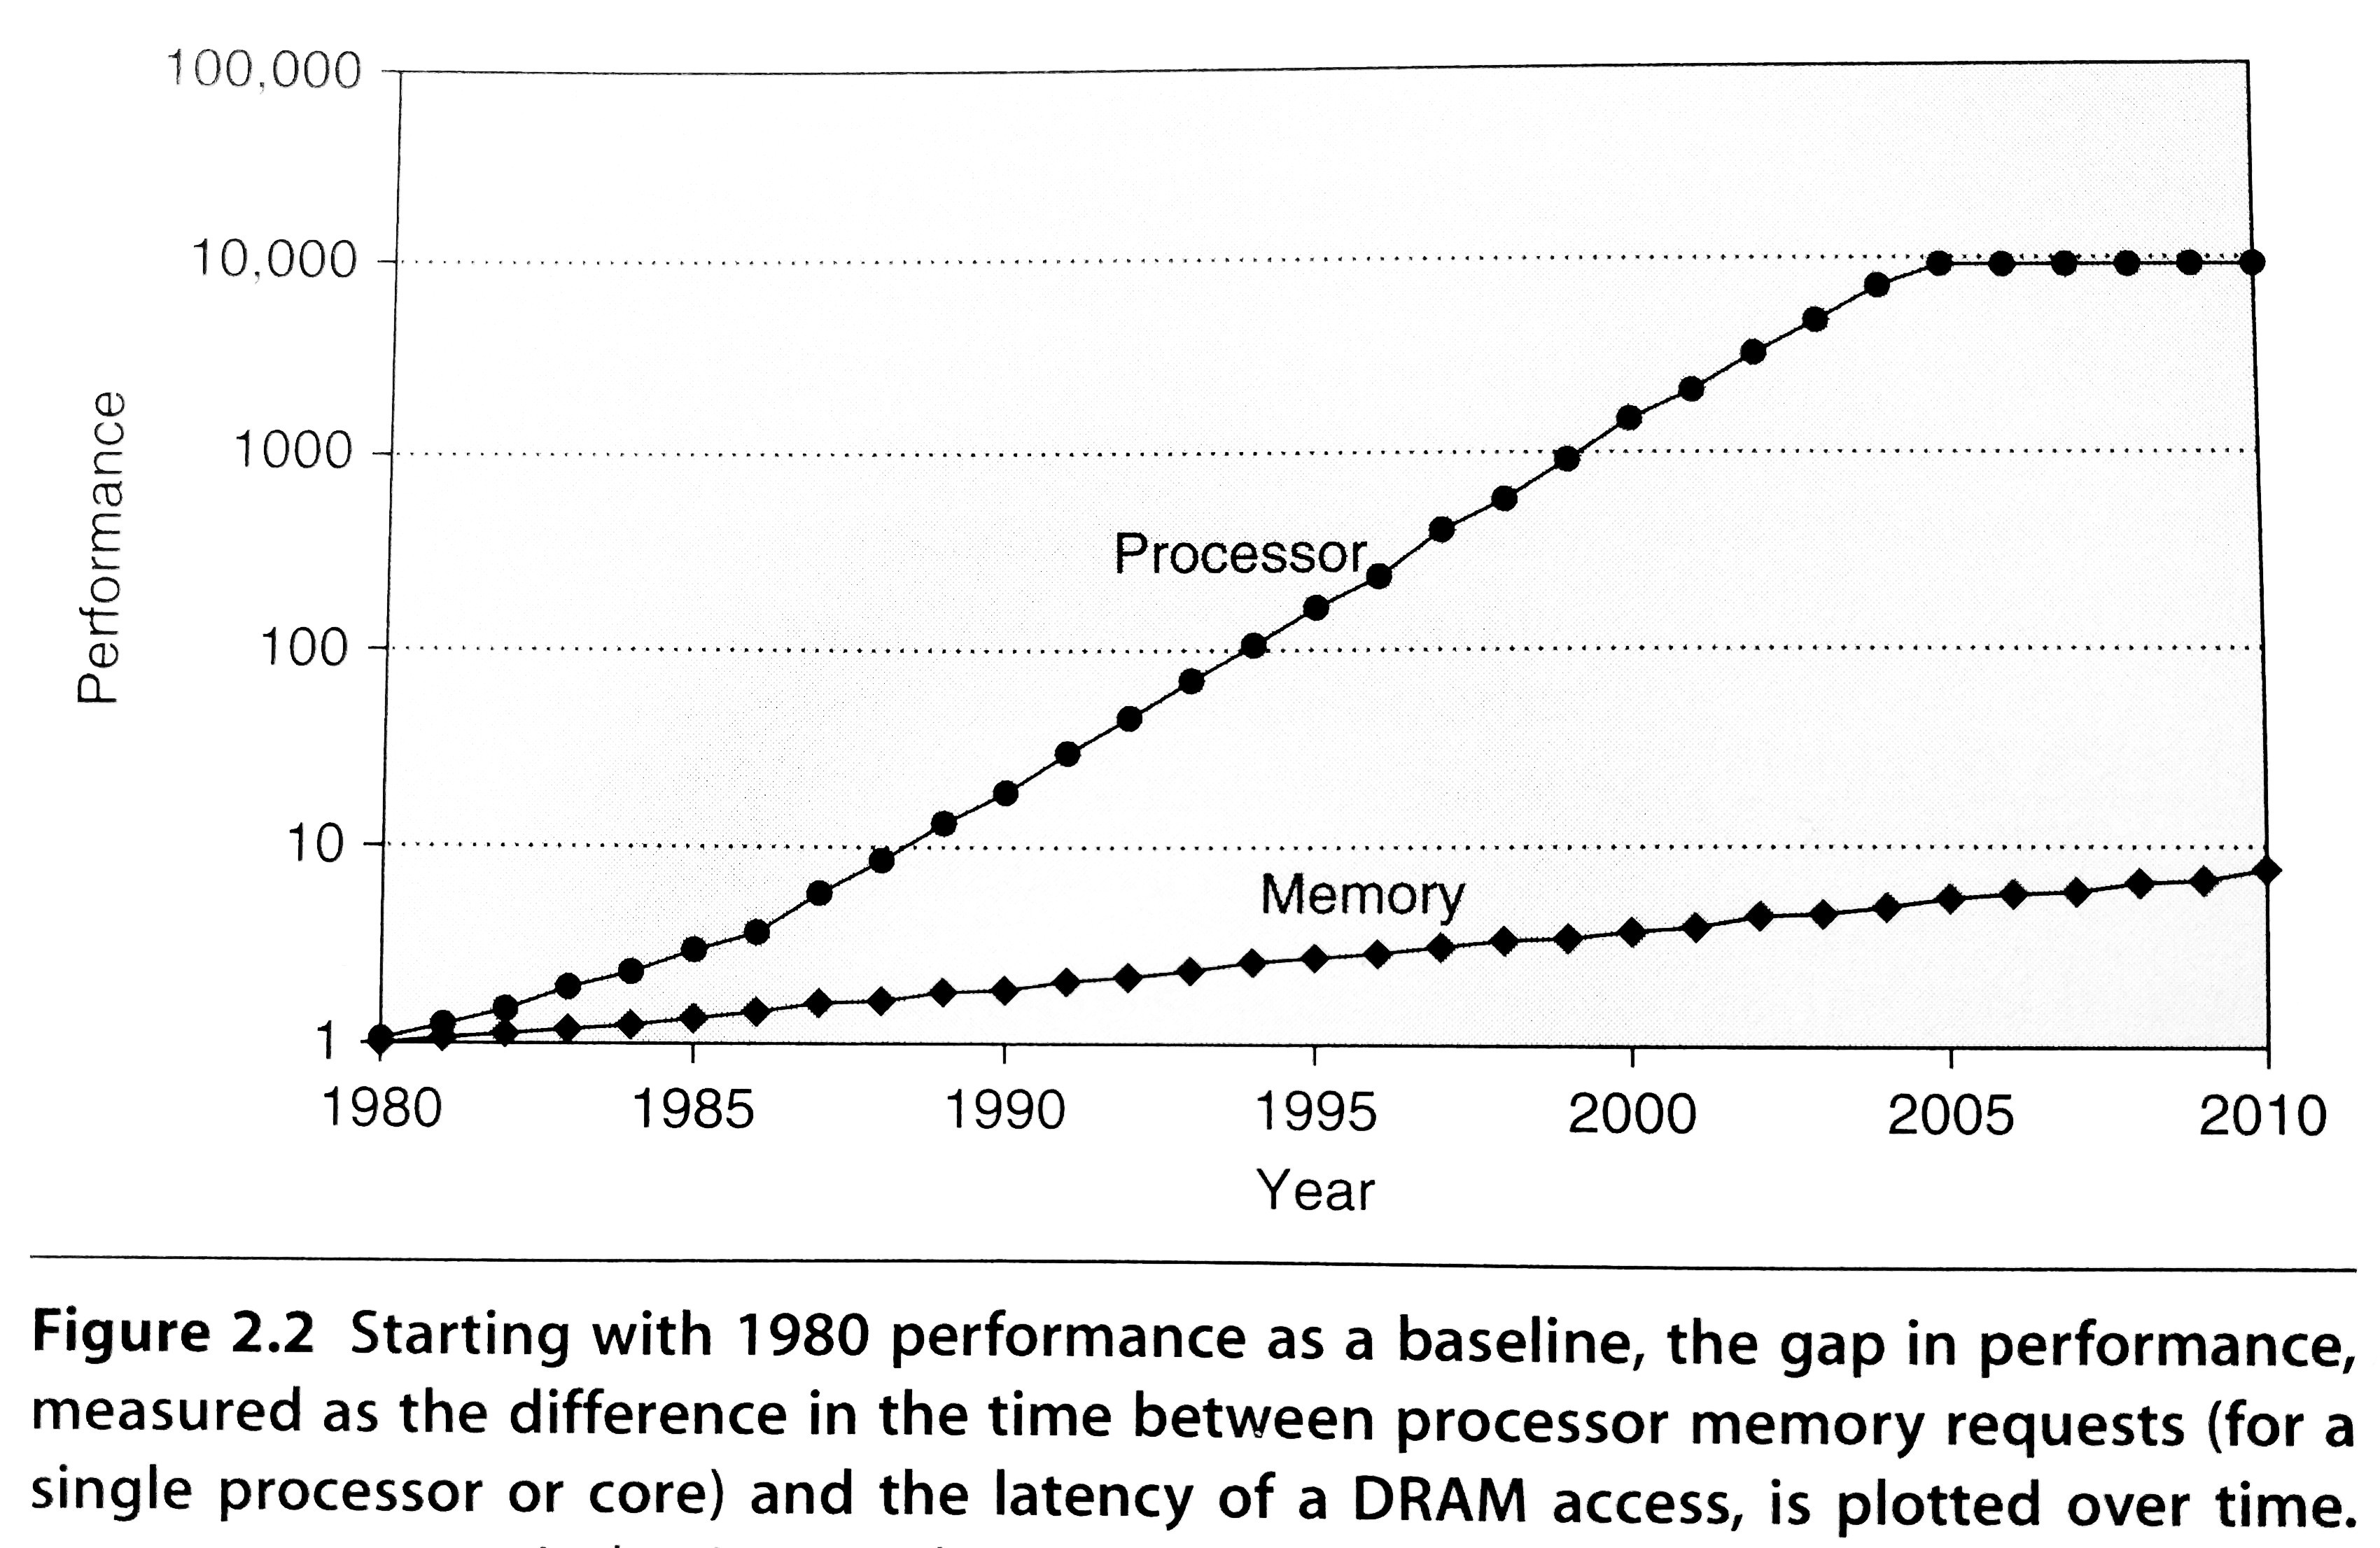
\includegraphics[width=\linewidth]{performance-gap.jpg}

\vspace{0.25 cm}
\begin{columns}
\column{0.2\linewidth}
\column{0.4\linewidth}
\tiny
From Hennessy \& Patterson, {\it Computer Architecture, A~Quantitative Approach.}

\column{0.25\linewidth}
\hspace{-0.5 cm}
\includegraphics[width=\linewidth]{hennessy-book.jpg}
\end{columns}
\end{columns}
\end{frame}

\begin{frame}[fragile]{Motivation}
\vspace{0.2 cm}
Columnar data representations are particularly complex for hierarchically nested data.

\vspace{0.25 cm}
\begin{columns}
\column{0.2\linewidth}
\column{0.3\linewidth}
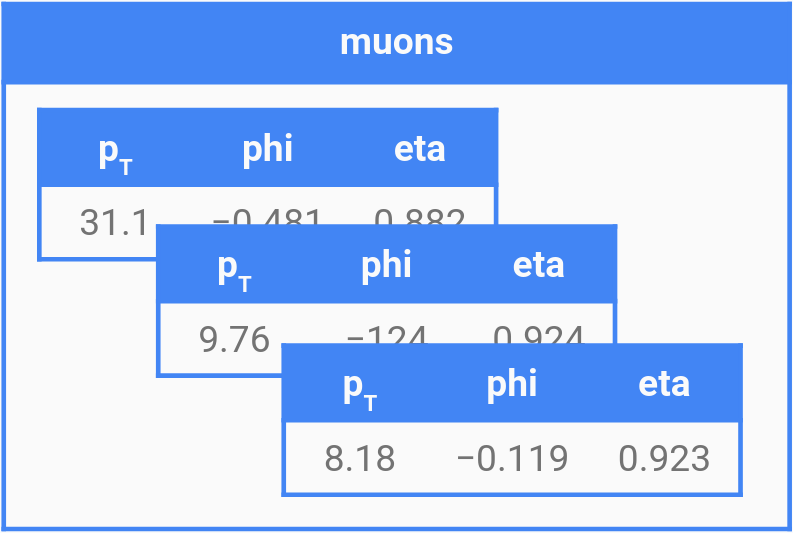
\includegraphics[width=\linewidth]{muons-as-objects.png}

\column{0.05\linewidth}
\centering vs

\column{0.3\linewidth}
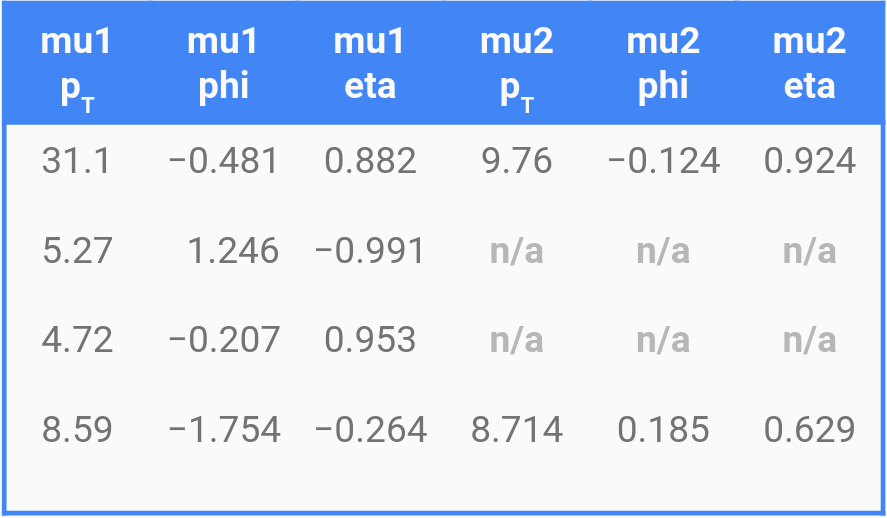
\includegraphics[width=\linewidth]{muons-as-a-table.png}
\column{0.2\linewidth}
\end{columns}

\vspace{0.25 cm}
\begin{uncoverenv}<2->
\scriptsize
\begin{Verbatim}[commandchars=\\\{\}]
[[Muon(\textcolor{darkgreen}{31.1}, \textcolor{darkorange}{-0.481}, \textcolor{blue}{0.882}), Muon(\textcolor{darkgreen}{9.76}, \textcolor{darkorange}{-0.124}, \textcolor{blue}{0.924}), Muon(\textcolor{darkgreen}{8.18}, \textcolor{darkorange}{-0.119}, \textcolor{blue}{0.923})],
 [Muon(\textcolor{darkgreen}{5.27}, \textcolor{darkorange}{1.246}, \textcolor{blue}{-0.991})],
 [Muon(\textcolor{darkgreen}{4.72}, \textcolor{darkorange}{-0.207}, \textcolor{blue}{0.953})],
 [Muon(\textcolor{darkgreen}{8.59}, \textcolor{darkorange}{-1.754}, \textcolor{blue}{-0.264}), Muon(\textcolor{darkgreen}{8.714}, \textcolor{darkorange}{0.185}, \textcolor{blue}{0.629})], ...
\end{Verbatim}
\end{uncoverenv}

\vspace{0.25 cm}
\begin{uncoverenv}<3->
\scriptsize
{\normalsize becomes four contiguous arrays, with ``offsets'' to express nesting structure:}

\vspace{0.25 cm}
\begin{tabular}{r l}
\small offsets &                    {\tt\scriptsize \ \ \ \ \ 0,\ \ \ \ \ \ \ \ \ \ \ \ \ \ \ \ \ \ \ \ \ \ 3,\ \ \ \ \ \ 4,\ \ \ \ \ \ 5,\ \ \ \ \ \ \ 7} \\
\small $p_T$ & \textcolor{darkgreen}{\tt\scriptsize \ \ 31.1,\ \ \ 9.76,\ \ \ 8.18,\ \ \ 5.27,\ \ \ 4.72,\ \ \ 8.59, 8.714} \\
\small phi &  \textcolor{darkorange}{\tt\scriptsize -0.481,\ -0.123,\ -0.119,\ \ 1.246,\ -0.207,\ -1.754,\ 0.185} \\
\small eta &        \textcolor{blue}{\tt\scriptsize \ 0.882,\ \ 0.924,\ \ 0.923,\ -0.991,\ \ 0.953,\ -0.264,\ 0.629} \\
\end{tabular}
\end{uncoverenv}
\end{frame}

\begin{frame}{This talk will be about}
\vspace{0.5 cm}
\Large
\begin{center}
\textcolor{darkblue}{Vertical performance from columnar data processing}

\vspace{0.5 cm}
{\it and}

\vspace{0.5 cm}
\textcolor{darkblue}{Convenient syntax for analysis scripts (in Python)}
\end{center}
\end{frame}

\begin{frame}[fragile]{Reading columnar data}
\vspace{0.5 cm}
The ROOT file format stores data in columns, but ROOT reads them back as C++ objects. If you want arrays for columnar data processing, you have to undo that step.

\vspace{0.5 cm}
\begin{uncoverenv}<2->
\hfill 
\includegraphics[height=2 cm]{uproot-logo.pdf}

\vspace{-2 cm}
uproot, an implementation of ROOT I/O in Python$+$Numpy, \\
reads TTree branches directly into Numpy arrays.
\end{uncoverenv}

\vspace{0.25 cm}
\begin{uncoverenv}<3->
\scriptsize
\begin{minted}{python}
>>> import uproot
>>> tree = uproot.open("NanoAOD-DYJetsToLL.root")["Events"]
>>> tree.array("Jet_pt")
jaggedarray([[],
             [29.96875   21.3125    19.671875  17.046875  15.4453125],
             [41.46875  27.625    22.       18.734375],
             ...,
             [34.03125  18.828125 18.359375],
             [42.78125   18.640625  17.640625  16.734375  15.921875  15.7890625],
             [23.75     23.640625 18.96875  ... 16.78125 16.28125 16.25   ]])
\end{minted}

\small
\vspace{0.1 cm}
Branches with nested structure, like {\tt\scriptsize std::vector<float>}, are read as columnar JaggedArrays.
\end{uncoverenv}
\end{frame}

\begin{frame}{Reading columnar data}
\vspace{0.5 cm}
Despite the fact that uproot is pure Python, throughput can exceed ROOT (C++) and root\_numpy (Cython) for baskets $\gtrsim$~20~kB.

\vspace{0.5 cm}
\begin{columns}
\column{0.5\linewidth}
\small
\mbox{ } \hfill \hfill speedup vs.\ ROOT \hfill \mbox{ }
\column{0.5\linewidth}
\small
\mbox{ } \hfill speedup vs.\ root\_numpy \hfill \hfill \mbox{ }
\end{columns}

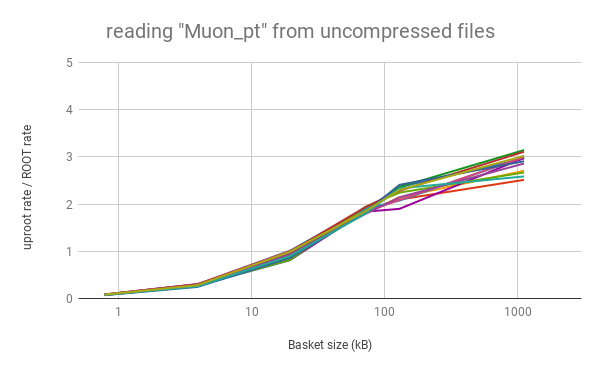
\includegraphics[width=0.5\linewidth]{root-none-muon.png}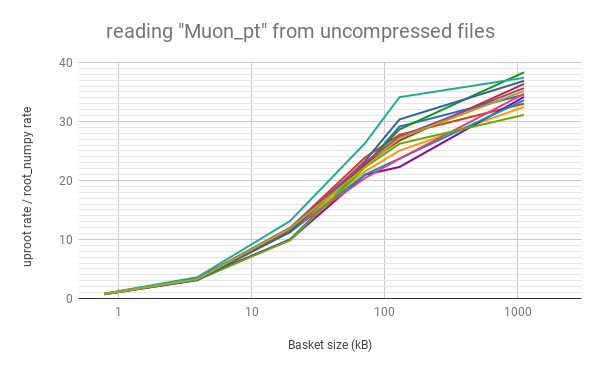
\includegraphics[width=0.5\linewidth]{rootnumpy-none-muon.png}

\vspace{0.25 cm}
This is because uproot is doing less work; only casting basket bytes as arrays.
\end{frame}

\begin{frame}[fragile]{Plotting columnar data}
\vspace{0.5 cm}
\hfill 
\includegraphics[height=1.5 cm]{histbook-logo.pdf}

\vspace{-1.7 cm}
The Numpy ecosystem lacks comprehensive, HEP-style \\
histogramming and ROOT is designed for events. \\
histbook provides array-at-a-time histogramming.

\vspace{0.25 cm}
\scriptsize
\begin{minted}{python}
>>> from histbook import *
>>> h = Hist(bin("x", 100, -5, 5), profile("x**2 + err"), profile("-x**3 + err"))
>>> h.fill(x=numpy.random.normal(0, 1, 10000),
...        err=numpy.random.normal(0, 5, 10000))
>>> beside(h.step("x"), h.marker("x", "x**2 + err"), h.marker("x", "-x**3 + err"))
\end{minted}

\mbox{ } \hfill 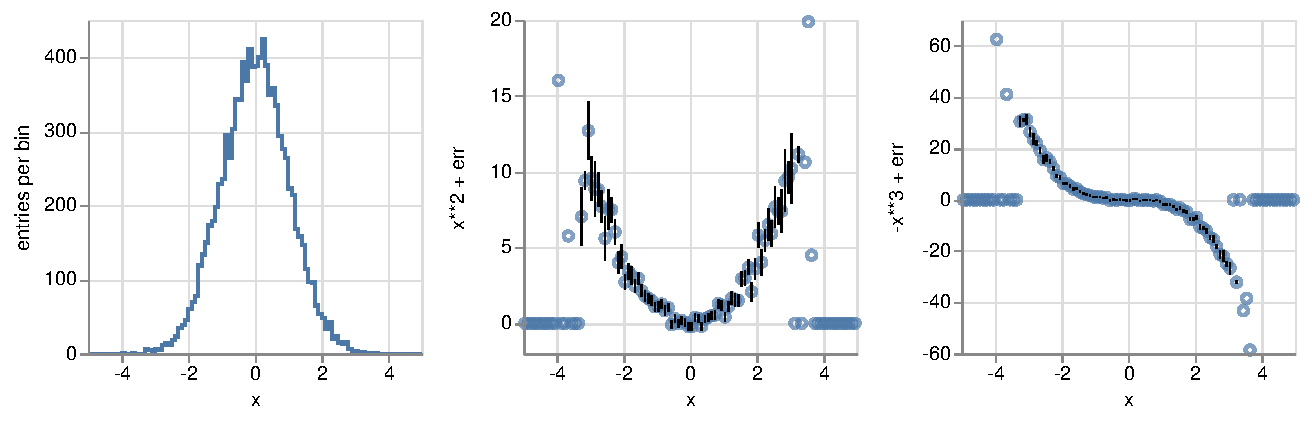
\includegraphics[width=0.7\linewidth]{histbook-example.pdf} \hfill \mbox{ }

\begin{minted}{python}
>>> h.project("x").root()
<ROOT.TH1D object at 0x62a1500>
\end{minted}
\end{frame}

\begin{frame}[fragile]{Manipulating columnar data}
\vspace{0.5 cm}
\hfill 
\includegraphics[height=2 cm]{awkward-logo.pdf}

\vspace{-2 cm}
The real problem, though, is {\it doing an analysis} on \\
columnar data. JaggedArrays are awkward:

\scriptsize
\begin{minted}{python}
>>> for event in range(event_muon_pts):
...     for pt, eta in zip(muon_pts[event], muon_etas[event]):
...         pz = pt * math.sinh(eta)
\end{minted}

\normalsize
especially if you want view all muon attributes collectively as an object (a jagged table).

\vspace{0.25 cm}
\begin{uncoverenv}<2->
awkward-array is a library in development to manipulate such structure like Numpy.

\scriptsize
\begin{minted}{python}
>>> # do all events and particles in one call because they have the same structure:
>>> events["muons"]["pt"] * numpy.sinh(events["muons"]["eta"])
<JaggedArray [[31.128 10.358 8.669] [-6.120] [5.211] [-2.295 5.850]] at 0x7fd394033080>
\end{minted}
\end{uncoverenv}

\begin{uncoverenv}<3->
\scriptsize
\begin{minted}{python}
>>> # add new attributes to a jagged table:
>>> events["muons"]["pz"] = events["muons"]["pt"] * numpy.sinh(events["muons"]["eta"])
>>> events["muons"][0].tolist()
[{"pt": 31.1, "phi": -0.481, "eta": 0.882, "pz": 31.128},
 {"pt": 9.76, "phi": -0.123, "eta": 0.924, "pz": 10.358},
 {"pt": 8.18, "phi": -0.119, "eta": 0.923, "pz": 8.669}]
\end{minted}
\end{uncoverenv}
\end{frame}

\begin{frame}[fragile]{Manipulating columnar data}
\vspace{0.5 cm}

awkward-array is a suite of \textcolor{darkblue}{composable}, high-level array types:
\begin{itemize}
\item \textcolor{darkblue}{jagged arrays:} for lists of lists of lists of lists\ldots
\item \textcolor{darkblue}{tables:} for sets of objects (may be jagged if composed with JaggedArray)
\item \textcolor{darkblue}{chunked:} for data that are not completely contiguous (i.e.\ ROOT baskets)
\item \textcolor{darkblue}{indexed:} for pointers, cross-references, dictionary-encoding, and event lists
\item \textcolor{darkblue}{masked:} for missing data (especially Apache Arrow bitmasks)
\item \textcolor{darkblue}{virtual:} for selective reading, e.g.\ only a few branches of a ROOT file
\item \textcolor{darkblue}{unions:} for polymorphism
\end{itemize}

\vspace{0.5 cm}
\begin{uncoverenv}<2->
The data model is very flexible, but the data are strictly columnar:

\scriptsize
\begin{minted}{python}
>>> import awkward
>>> columnar_data = awkward.fromiter([1, 2, 3.3, None, [4, 5], {"six": 6}])
>>> columnar_data.tolist()
[1.0, 2.0, 3.3, None, [4, 5], {'six': 6}]
\end{minted}
\end{uncoverenv}
\end{frame}

\begin{frame}[fragile]{Manipulating columnar data}
\vspace{0.3 cm}

\hfill 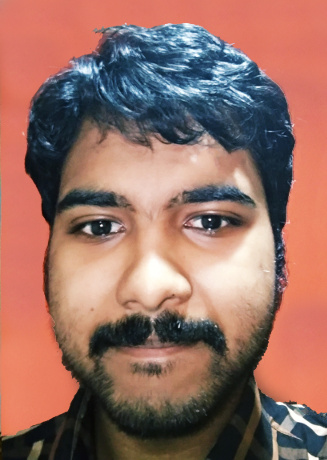
\includegraphics[height=3 cm]{jaydeep.jpg}

\vspace{-3 cm}
\textcolor{darkblue}{Jaydeep Nandi}, our Google Summer of Code student, is investigating \\
vectorized algorithms to replace for-loop manipulations.

\vspace{0.1 cm}
\scriptsize
\begin{minted}{python}
>>> # broadcast per-event attributes to per-particle attributes:
>>> events["MET"]["phi"] - events["jets"]["phi"]

>>> # apply cuts with Numpy-like masks:
>>> events_with_two = events["muons"][events["muons"].counts >= 2]

>>> # explode to event-wise pairs of muons:
>>> pairs = events_with_two.pairs()
>>> pairs
<JaggedArray [[<Pair 0> <Pair 1> <Pair 2>] [<Pair 3>]] at 0x7fd394033080>
>>> pairs[0][0].tolist()
{"_0": {"pt": 31.1, "phi": -0.481, "eta": 0.882, "pz": 31.128},
 "_1": {"pt": 9.76, "phi": -0.123, "eta": 0.924, "pz": 10.358}}

>>> m1, m2 = pairs["_0"], pairs["_1"]
>>> mass = numpy.sqrt(2*m1["pt"]*m2["pt"]*(
...     numpy.cosh(m1["eta"] - m2["eta"]) - numpy.cos(m1["phi"] - m2["phi"])))
\end{minted}

\normalsize
\vspace{0.1 cm}
Incidentally, anything that can be expressed this way is ripe for GPU vectorization.
\end{frame}

\begin{frame}[fragile]{Manipulating columnar data}
\vspace{0.5 cm}

\hfill 
\includegraphics[height=2 cm]{numba-logo.png}

\vspace{-2 cm}

Analysis functions that can't be expressed as explosions, masks, and \\
reductions can at least be JIT-compiled. Numba (from Anaconda) is \\
a JIT-compiler for Python code.

\vspace{0.5 cm}
I implemented awkward-array's predecessor, OAMap, as a Numba extension to get $\sim$500$\times$ speedups. I will apply the same techniques to the new library.

\vspace{0.5 cm}
\begin{columns}[t]
\column{0.46\linewidth}
\underline{Runs in 12.9 seconds}

\scriptsize
\vspace{2\baselineskip}
\begin{minted}{python}
def run(pz, events):
  k = 0
  for event in events:
    for muon in event.muons:
      pz[k] = muon.pt * math.sinh(muon.eta)
      k += 1
\end{minted}

\column{0.46\linewidth}
\underline{Runs in 0.023 seconds}

\scriptsize
\begin{minted}{python}
import numba
@numpy.jit
def run(pz, events):
  k = 0
  for event in events:
    for muon in event.muons:
      pz[k] = muon.pt * math.sinh(muon.eta)
      k += 1
\end{minted}
\end{columns}
\end{frame}

\begin{frame}{What does all of this buy us?}
\vspace{0.3 cm}
\begin{columns}
\column{1.15\linewidth}
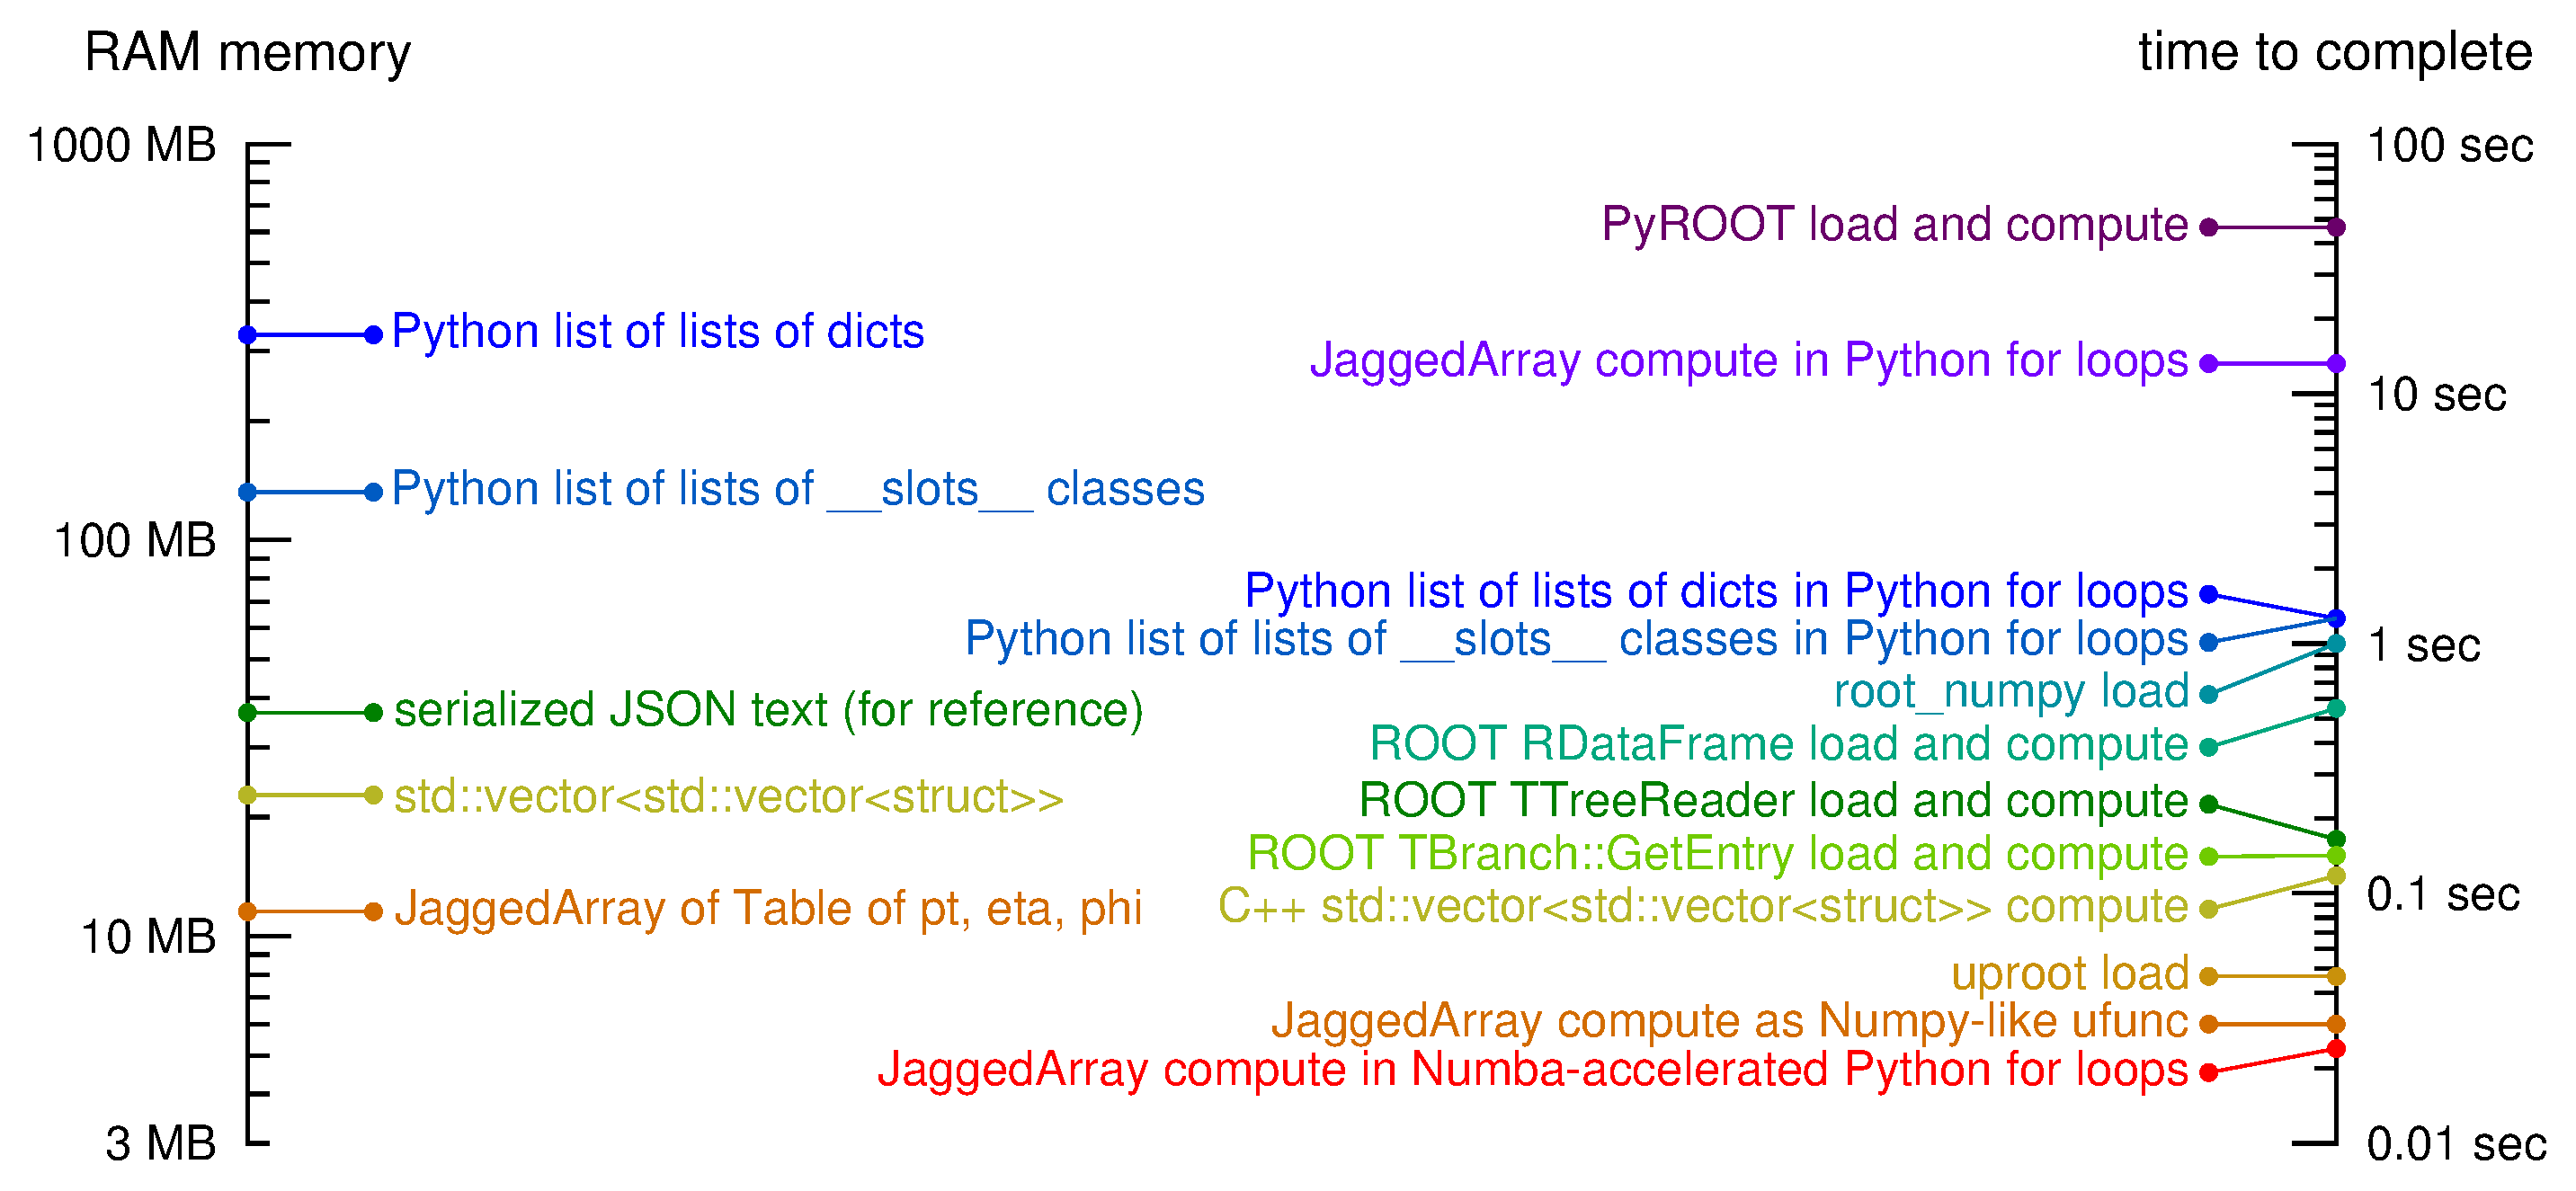
\includegraphics[width=\linewidth]{logscales.pdf}
\end{columns}
\end{frame}

\begin{frame}{What does all of this buy us?}
\vspace{0.5 cm}
\scriptsize

\begin{columns}
\column{1.1\linewidth}
\begin{columns}
\column{0.38\linewidth}
\begin{tabular}{r p{0.9\linewidth}}
& \textcolor{darkblue}{\small\underline{RAM memory occupied by data (MB)}} \\
& \\
311.95 & \textcolor{pythoncolor}{Python list of lists of dicts} \\
215.11 & \textcolor{rootnpcolor}{root\_numpy's array of arrays} \\
139.79 & \textcolor{pythoncolor}{Python list of lists of {\tt\scriptsize \_\_slots\_\_} classes} \\
& \\
 37.19 & \textcolor{gray}{serialized JSON text (for reference)} \\
& \\
 22.38 & \textcolor{cppcolor}{\tt\scriptsize std::vector<std::vector<struct>>} \\
 11.67 & \textcolor{mycolor}{JaggedArray of Table of pt, eta, phi} \\
& \\
& \textcolor{gray}{\scriptsize 1 MB = 1024$^2$ bytes} \\
& \textcolor{gray}{\scriptsize 701,716 events containing 552,056 muons} \\
& \textcolor{gray}{\scriptsize storing pt, eta, phi as float32} \\
\end{tabular}

\vspace{2.3 cm}

\column{0.6\linewidth}
\begin{tabular}{r p{0.9\linewidth}}
& \textcolor{darkblue}{\small\underline{time to complete load, compute, or both (sec)}} \\
& \\
45.9\textcolor{white}{00} & \textcolor{rootcolor}{PyROOT load and compute} \\
12.9\textcolor{white}{00} & \textcolor{mycolor}{JaggedArray compute in Python for loops} \\
& \\
1.67\textcolor{white}{0} & \textcolor{rootnpcolor}{root\_numpy compute in loop over ufuncs} \\
 1.24\textcolor{white}{0} & \textcolor{pythoncolor}{Python list of lists of dicts in Python for loops} \\
 1.23\textcolor{white}{0} & \textcolor{pythoncolor}{Python list of lists of {\tt\scriptsize \_\_slots\_\_} classes in Python for loops} \\
& \\
 1.01\textcolor{white}{0} & \textcolor{rootnpcolor}{root\_numpy load} \\
& \\
 0.538 & \textcolor{rootcolor}{ROOT RDataFrame load and compute} \\
 0.164 & \textcolor{rootcolor}{ROOT TTreeReader load and compute} \\
 0.142 & \textcolor{rootcolor}{ROOT TBranch::GetEntry load and compute} \\
 0.113 & \textcolor{cppcolor}{{\tt\scriptsize std::vector<std::vector<struct>>} compute} \\
& \\
 0.047 & \textcolor{mycolor}{uproot load} \\
 0.030 & \textcolor{mycolor}{JaggedArray compute as Numpy-like ufunc} \\
 0.023 & \textcolor{mycolor}{JaggedArray compute in Numba-accelerated Python for loops} \\
& \\
& \textcolor{gray}{\scriptsize all with warmed disk cache} \\
\end{tabular}
\end{columns}
\end{columns}
\end{frame}

\begin{frame}{Conclusions}
\vspace{0.5 cm}
\large
\begin{itemize}\setlength{\itemsep}{0.5 cm}
\item Python has a model for expressing operations on columnar data: Numpy.
\item We must extend that model for the variable-length structures that are ubiquitous in HEP data.
\item Opportunities for fundamental work: e.g.\ how do you do gen/reco jet matching in vectorized instructions?
\item Can hold more data in memory at a time than non-columnar C++ structures and process it faster, without leaving Python.
\end{itemize}
\end{frame}

\begin{frame}
\huge
\begin{center}
\textcolor{darkblue}{Backup}
\end{center}
\end{frame}

\begin{frame}[fragile]{JaggedArray compute in Python for loops}
\vspace{0.3 cm}
\scriptsize
\begin{minted}{python}
%%timeit
k = 0
for event in events:
    for muon in event:
        pz[k] = muon.pt * math.sinh(muon.eta)
        k += 1
\end{minted}

\vspace{0.5 cm}
\hfill\begin{minipage}{0.6\linewidth}
{\normalsize \ldots with Numba acceleration:}
\begin{minted}{python}
import numba

@numpy.jit
def callme(pz, events):
    k = 0
    for event in events:
        for muon in event:
            pz[k] = muon.pt * math.sinh(muon.eta)
            k += 1

%%timeit
callme(pz, events)
\end{minted}
\end{minipage}
\end{frame}

\begin{frame}[fragile]{JaggedArray and root\_numpy ufuncs}
\scriptsize
{\normalsize JaggedArray compute as Numpy-like ufunc:}
\begin{minted}{python}
import numpy

%%timeit
pz = events["pt"] * numpy.sinh(events["eta"])
\end{minted}

\vspace{0.5 cm}
\hfill\begin{minipage}{0.6\linewidth}
{\normalsize root\_numpy compute in loop over ufuncs:}
\begin{minted}{python}
%%timeit
k = 0
for event in events:
    pt = event["Muon_pt"]
    eta = event["Muon_eta"]
    pz[k : k + len(pt)] = pt * numpy.sinh(eta)
    k += len(pt)
\end{minted}
\end{minipage}
\end{frame}

\begin{frame}[fragile]{Python list of lists of dicts/classes compute in Python for loops}
\scriptsize
\begin{columns}[t]
\column{0.5\linewidth}
\begin{minted}{python}
from math import sinh

events = [
    [],
    [{"pt": 129.8,
      "eta": -1.006,
      "phi": -0.581},
     {"pt": 73.08,
      "eta": -0.719,
      "phi": -1.51}],
    ...
    ]

%%timeit
k = 0
for event in events:
    for muon in event:
        pz[k] = (muon["pt"] *
                 sinh(muon["eta"]))
        k += 1
\end{minted}

\column{0.5\linewidth}
\begin{minted}{python}
class Muon(object):
    __slots__ = ["pt", "eta", "phi"]
    def __init__(self, pt, eta, phi):
        self.pt = pt
        self.eta = eta
        self.phi = phi

events = [
    [],
    [Muon(129.8, -1.006, -0.581),
     Muon(73.08, -0.719, -1.51)],
    ...
    ]

%%timeit
k = 0
for event in asobjs:
    for muon in event:
        pz[k] = (muon.pt *
                 sinh(muon.eta))
        k += 1
\end{minted}
\end{columns}
\end{frame}

\begin{frame}[fragile]{root\_numpy load and uproot load}
\scriptsize
\begin{minted}{python}
import ROOT
import root_numpy

file = ROOT.TFile("NanoAOD-DYJetsToLL.root")
tree = file.Get("tree")

%%timeit
root_numpy.tree2array(tree, ["Muon_pt", "Muon_eta", "Muon_phi"])




import uproot
tree = uproot.open("NanoAOD-DYJetsToLL.root")["tree"]

%%timeit
pt, eta, phi = tree.arrays(["Muon_pt", "Muon_eta", "Muon_phi"], outputtype=tuple)
\end{minted}
\end{frame}

\begin{frame}[fragile]{PyROOT load and compute}
\scriptsize
\begin{minted}{python}
import math
import numpy
import ROOT

file = ROOT.TFile("NanoAOD-DYJetsToLL.root")
tree = file.Get("tree")

tree.SetBranchStatus("*", 0)
tree.SetBranchStatus("nMuon", 1)
tree.SetBranchStatus("Muon_pt", 1)
tree.SetBranchStatus("Muon_eta", 1)

pz = numpy.empty(552056, dtype=numpy.float32)

%%timeit
k = 0
for event in tree:
    for pt, eta in zip(event.Muon_pt, event.Muon_eta):
        pz[k] = pt * math.sinh(eta)
        k += 1
\end{minted}
\end{frame}

\begin{frame}[fragile]{ROOT RDataFrame load and compute}
\vspace{0.1 cm}
\scriptsize
\begin{columns}
\column{1.05\linewidth}
\begin{minted}{c++}
#include <ctime>
#include <sys/time.h>
struct timeval starttime, endtime;

auto file = TFile::Open("NanoAOD-DYJetsToLL.root")
ROOT::RDataFrame rdf("tree", file);

TTree* tree; file->GetObject("tree", tree);   // perhaps unnecessary, but just in case...
tree->SetBranchStatus("*", 0);
tree->SetBranchStatus("nMuon", 1);
tree->SetBranchStatus("Muon_pt", 1);
tree->SetBranchStatus("Muon_eta", 1);

float pz[552056];
gettimeofday(&starttime, 0);
int k = 0;
rdf.Foreach([&k](ROOT::VecOps::RVec<float> Muon_pt, ROOT::VecOps::RVec<float> Muon_eta) {
    for (int i = 0;  i < Muon_pt.size();  i++) {
        pz[k]= Muon_pt[i] * sinh(Muon_eta[i]);
        k++;
    }
}, {"Muon_pt", "Muon_eta"});
gettimeofday(&endtime, 0);
\end{minted}
\end{columns}
\end{frame}

\begin{frame}[fragile]{ROOT TTreeReader load and compute}
\scriptsize
\begin{columns}
\column{1.05\linewidth}
\begin{minted}{c++}
#include <ctime>
#include <sys/time.h>
struct timeval starttime, endtime;

auto file = TFile::Open("NanoAOD-DYJetsToLL.root")
TTree* tree; file->GetObject("tree", tree);   // perhaps unnecessary, but just in case...
tree->SetBranchStatus("*", 0);
tree->SetBranchStatus("nMuon", 1);
tree->SetBranchStatus("Muon_pt", 1);
tree->SetBranchStatus("Muon_eta", 1);

TTreeReader reader("tree", file);
TTreeReaderArray<float> pt(reader, "Muon_pt");
TTreeReaderArray<float> eta(reader, "Muon_eta");

gettimeofday(&starttime, 0);
int k = 0;
while (reader.Next()) {
    for (int i = 0;  i < pt.GetSize();  i++) {
        pz[k] = pt[i] * sinh(eta[i]);
        k++;
    }
}
gettimeofday(&endtime, 0);
\end{minted}
\end{columns}
\end{frame}

\begin{frame}[fragile]{ROOT TBranch::GetEntry load and compute}
\vspace{0.2 cm}
\scriptsize
\begin{columns}
\column{1.1\linewidth}
\begin{minted}{c++}
#include <ctime>
#include <sys/time.h>
struct timeval starttime, endtime;

auto file = TFile::Open("NanoAOD-DYJetsToLL.root")
TTree* tree; file->GetObject("tree", tree);

UInt_t nMuon; float pts[10]; float etas[10];
TBranch* nbranch = tree->GetBranch("nMuon");       tree->SetBranchAddress("nMuon", &nMuon);
TBranch* ptbranch = tree->GetBranch("Muon_pt");    tree->SetBranchAddress("Muon_pt", pts);
TBranch* etabranch = tree->GetBranch("Muon_eta");  tree->SetBranchAddress("Muon_eta", etas);

gettimeofday(&starttime, 0);
int k = 0;
for (int i = 0;  i < 701716;  i++) {
    // TBranch::GetEntry, rather than TTree::GetEntry, avoids a loop over branches
    nbranch->GetEntry(i);    ptbranch->GetEntry(i);    etabranch->GetEntry(i);
    for (int j = 0;  j < nMuon;  j++) {
        pz[k] = pts[j] * sinh(etas[j]);
        k++;
    }
}
gettimeofday(&endtime, 0);
\end{minted}
\end{columns}
\end{frame}

\begin{frame}[fragile]{{\tt std::vector<std::vector<struct>>}}
\vspace{0.3 cm}
\scriptsize
\begin{minted}{c++}
struct Muon {
    float pt;
    float eta;
    float phi;
};

struct Event {
    std::vector<Muon> muons;
};

auto events = // std::vector<std::vector<Muon>>, filled with push_back

gettimeofday(&starttime, 0);
int k = 0;
for (int i = 0;  i < events.size();  i++) {
    for (int j = 0;  j < events[i].muons.size();  j++) {
        pz[k] = events[i].muons[j].pt * sinh(events[i].muons[j].eta);
        k++;
    }
}
gettimeofday(&endtime, 0);
\end{minted}
\end{frame}

\end{document}
